\section{Methodology}
\label{sec:method}
% include the figures path relative to the master file
\graphicspath{ {./content/method/figures/} }

% \begin{figure}[t]
%     \centering
%     \begin{subfigure}[b]{0.30\textwidth}
%         \centering
%         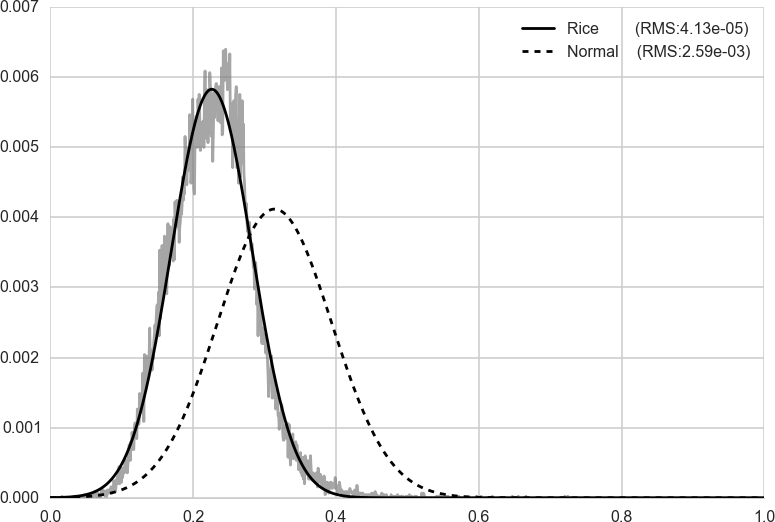
\includegraphics[width=\textwidth]{03}
%     \end{subfigure}
%     \hfill
%     \begin{subfigure}[b]{0.30\textwidth}
%         \centering
%         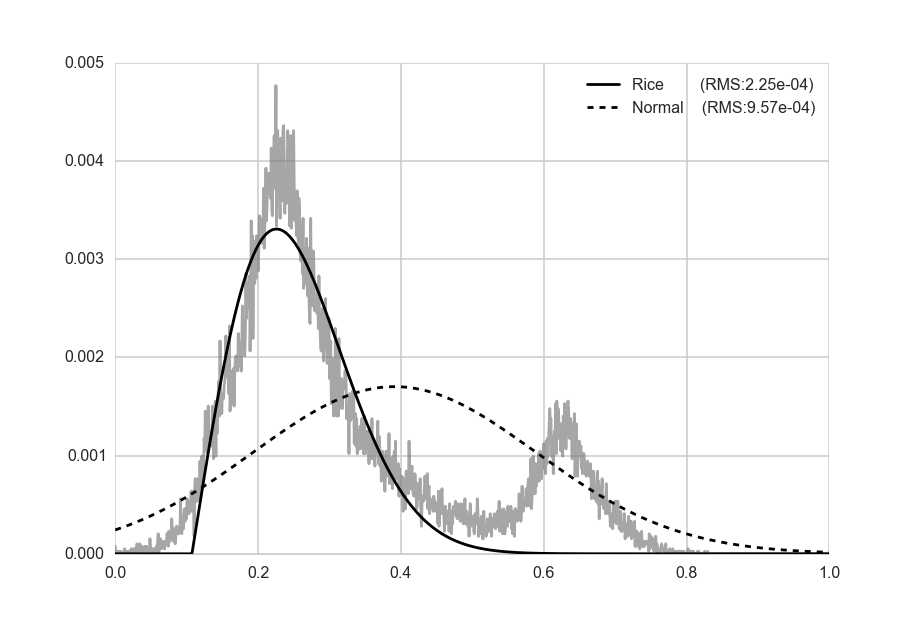
\includegraphics[width=\textwidth]{06}
%     \end{subfigure}
%     \hfill
%     \begin{subfigure}[b]{0.30\textwidth}
%         \centering
%         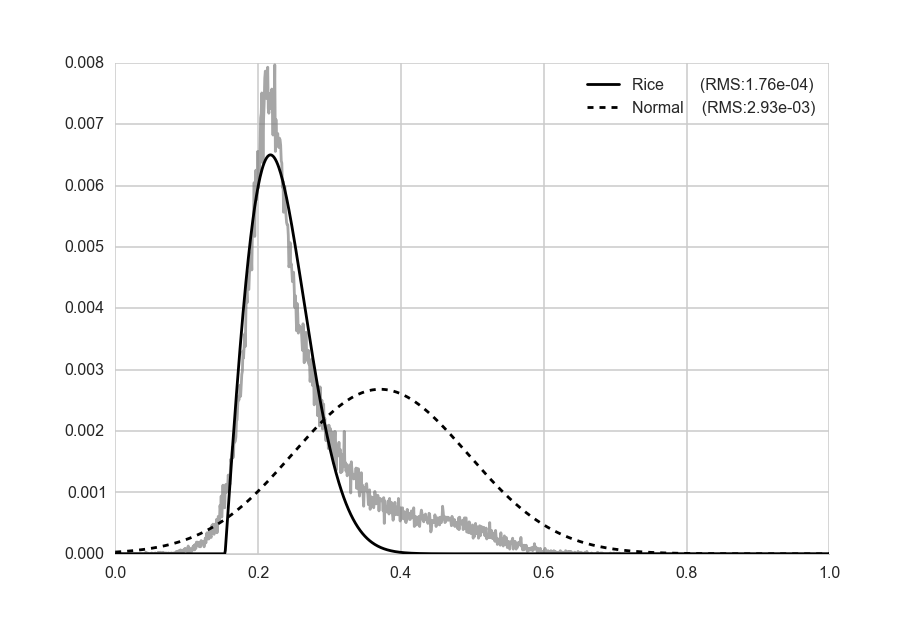
\includegraphics[width=\textwidth]{14}
%     \end{subfigure}
%     \caption {Fitting differences}
%     \label{fig:rice-norm-diff}
% \end{figure}

\subsection{Normalization using Rician \textit{a priori}}

As stated in~Sect.\,\ref{sec:intro}, proper normalization of the \ac{mri} data during pre-processing is a key problem that has been addressed using parametric and non-parametric strategies.
We believe that normalizing \ac{mri} data using a parametric model based on a Rician distribution would improve the results for the parametric case.
Expecting this improvement by changing the data model from the widely used Gaussian distribution to Rician distribution is reasonable. 
Indeed, Bernstein\,\textit{et al.}~\cite{bernstein1989improved} state that \ac{mri} data theoretically follows a Rayleigh distribution for a low \ac{snr} scenarios while it appears closer to a Gaussian distribution when the \ac{snr} increases.
Figure~\ref{fig:fitting} shows the intensity spectrum for some \ac{mri} prostate data as well as the fitted Gaussian and Rician distributions.
A qualitative assessment of the underlying distribution is performed by overlying the fitted distribution, while quantitative results of the fitting are given in terms of \ac{rms}.
It can be highlighted that the Rician model better fits the data than the Gaussian model.

\begin{figure*}
  \centering
  \subfloat[][]{
    \label{fig:p1}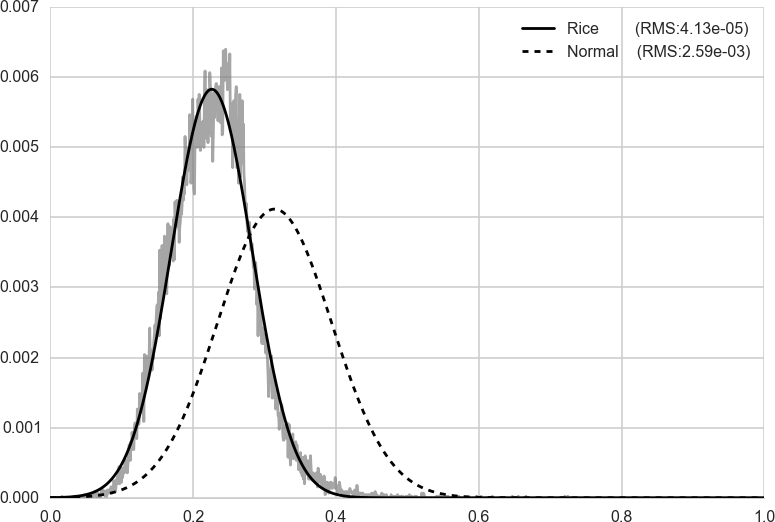
\includegraphics[width=0.48\textwidth]{03}}\hfill
  \subfloat[][]{
    \label{fig:p2}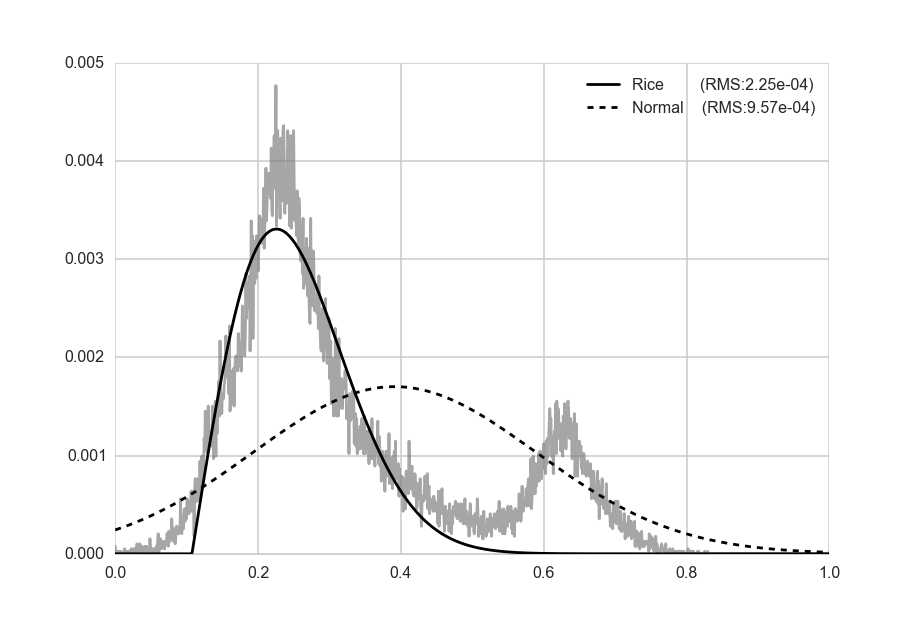
\includegraphics[width=0.48\textwidth]{06}}\hfill
%  \subfloat[][]{
%    \label{fig:p3}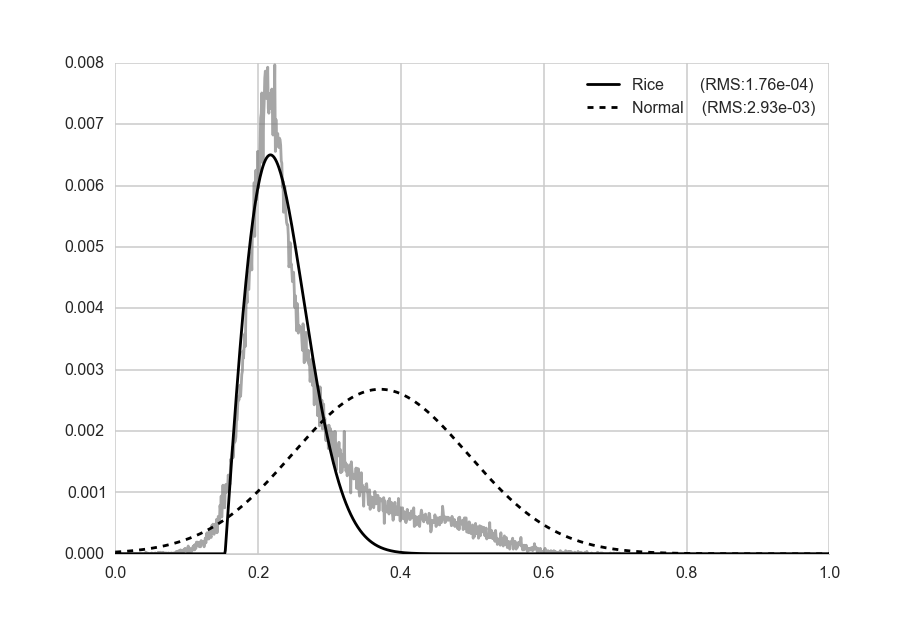
\includegraphics[width=0.3\textwidth]{14}}
  \caption{Visual evaluation of the goodness of fitting using Rician and Gaussian distribution.}
  \label{fig:fitting}
\end{figure*}

The normalization is carried out as: 
(i) fit a Rician model to each prostate \ac{pdf} using non-linear least squares minimization; 
(ii) compute the mean (see~Eq.\,\eqref{eq:meanr}) and variance (see~Eq.\,\eqref{eq:var}) of the Rician model;
(iii) normalize the entire data using the \textit{z-score} similarly as in~Eq.\,\eqref{eq:zscore}.

\begin{equation}
  \mu_{r} = \sigma  \sqrt{\frac{\pi}{2}}\,\,L_{1/2}(-\frac{\nu^2}{2\sigma^2})  \ ,
  \label{eq:meanr}
\end{equation}

\begin{equation}
  \sigma_{r} = 2\sigma^2+\nu^2-\frac{\pi\sigma^2}{2}L_{1/2}^2\left(\frac{-\nu^2}{2\sigma^2}\right)  \ ,
  \label{eq:var}
\end{equation}

\noindent where $\nu$ and $\sigma$ are the distance between the reference point and the center of the bivariate distribution and the scale, respectively; $L_{1/2}$ denotes a Laguerre polynomial.

\subsection{Normalization using generative models in functional data analysis}

Srivastava\,\textit{et al.}~\cite{Srivastava2011} have proposed a generic method to register functional data, without any assumption regarding the models of different functions. 
This framework (see Sect.\,\ref{sec:regfra}) relies on the \ac{srsf} representation (see Sect.\,\ref{sec:srsf}) which transforms the Fisher-Rao metric into the conventional $\mathbb{L}^2$ metric, and thus allows to define a cost function corresponding to an Euclidean distance between two functions in this new representation.

\subsubsection{\acl*{srsf} representation} \label{sec:srsf}

In the proposed registration framework of functional data, two function $f_1$ and $f_2$ are registered by composing $f_2$ with a warping function $\gamma$ such that:

\begin{equation}
  \argmin_{\gamma \in \Gamma} D_{FR}(f_1, (f_2 \circ \gamma)) \ ,
  \label{eq:regfun}
\end{equation}

\noindent where $D_{FR}$ is the Fisher-Rao distance and $\Gamma$ is the set of all the functions $\gamma$.

The \Ac{srsf} representation is used to transform the functions and register them into this space. The \ac{srsf} of a function $f$ is defined as:

\begin{equation}
  q(t) = \sign(\dot{f}(t))\sqrt{|\dot{f}(t)|} \ ,
  \label{eq:srsf}
\end{equation}

\noindent where $\dot{f}(t)$ corresponds to the derivative of $f$.

The major property of the \ac{srsf} representation used in the registration framework is the following: the composition of a function $f$ with a warping function $\gamma$ (i.e., $f \circ \gamma$) is equivalent to Eq.\,\eqref{eq:warp}, using the \ac{srsf} representation.

\begin{equation}
  \tilde{q}(t) = (q(t) \circ \gamma) \sqrt{\dot{\gamma}} \ ,
  \label{eq:warp}
\end{equation}

\noindent where $\dot{\gamma}$ is the derivative of $\gamma$.

Using this property, a cost function (named amplitude or $y$-distance) is defined to measure the similarity between two functions $f_1$ and $f_2$, expressed as in Eq.\,\eqref{eq:cf}

\begin{equation}
  D_y(f_1, f_2) = \underset{\gamma \in \Gamma}{\infspie} \| q_1 - (q_2 \circ \gamma) \sqrt{\dot{\gamma}} \| \ .
  \label{eq:cf}
\end{equation}

\subsubsection{Registration framework}\label{sec:regfra}

The registration framework consists into two steps. First, an initialization in which the Karcher mean $\mu_f$ is computed as in Eq.\,\eqref{eq:mean}

\begin{equation}
  \mu_f = \argmin_{f \in \mathcal{F}} \sum_{i = 1}^{n} D_y(f, f_i)^2 \ .
  \label{eq:mean}
\end{equation}

Then, for each function $f_i$: 
(i) compute $\gamma_{i}^{*}$ as in Eq.\,\eqref{eq:warpi}; 
(ii) compute $\tilde{q}_i$ as in Eq.\,\eqref{eq:warp};
(iii) update $\mu_f$ as in Eq.\,\eqref{eq:mean} by replacing $f_i$ by $\tilde{f_i}$, using $\tilde{q}_i$.

\begin{equation}
  \gamma_{i}^{*} = \argmin_{\gamma \in \Gamma} \sum_{i = 1}^{n} D_y(\mu_f, f_i)^2 \ ,
  \label{eq:warpi}
\end{equation}

\noindent where $n$ is the total number of functions to be aligned.

This step is iteratively performed based on the gradient of the cost function given in Eq.\,\eqref{eq:mean}. We refer the reader to the work of Srivastava\,\textit{et al.}~\cite{Srivastava2011} for more detailed discussion.

%%% Local Variables: 
%%% mode: latex
%%% TeX-master: "../../master"
%%% End: 

